\section{Loi normale}
La loi la plus utilis\'ee pour d\'ecrire des ph\'enom\`enes par une variable al\'eatoire continue est la loi normale. Par exemple, la description du poids, de la taille, du remplissage de r\'ecipients, ... Cette loi est abondamment utilis\'ee lors de l'inf\'erence statistique.

La repr\'esentation graphique de la loi normale est une courbe en forme de cloche, sym\'etrique.
$$\includegraphics[scale=0.5]{norm_0_1}$$

\begin{defi}
La \emph{densit\'e de probabilit\'e normale} s'exprime par
$$f(x)=\frac{1}{\sigma\sqrt{2\pi}}e^{-\frac{(x-\mu)^2}{2\sigma^2}}$$
o� $\mu$ est la moyenne et $\sigma$ est l'\'ecart type
\end{defi}

La loi normale, not\'ee $\mathcal{N}(\mu,\sigma^2)$, comporte deux param\`etres $\mu$ et $\sigma^2$, qui d\'eterminent la position et la forme de la distribution. Il existe donc une famille de lois normales, et non pas une seule, qui se diff\'erencient par leur moyenne et leur \'ecart type.

\begin{pro}
\begin{itemize}
	\item Le point le plus \'elev\'e de la courbe normale correspond \`a la moyenne, qui est aussi la m\'ediane et le mode de la distribution.
  \item La distribution normale \'etant sym\'etrique, son  coefficient d'asym\'etrie (skewness) est nul.
  \item L'\'ecart type d\'etermine la largeur de la courbe. Plus sa valeur est \'elev\'ee, plus la courbe sera large et aplatie.
	\item La variable al\'eatoire associ\'ee peut prendre n'importe quelle valeur r\'eelle dans $]-\infty, \infty [$.
\end{itemize}
\end{pro}

La probabilit\'e est repr\'esent\'ee par l'aire sous la courbe de densit\'e $f(x)$. L'aire totale vaut 1 car il s'agit d'une probabilit\'e. Comme la loi normale est sym\'etrique, la probabilit\'e $P(X\leq\mu)=P(X\geq\mu)=0.5$, et par cons\'equent
$$P(X\leq x) = 1-P(X\geq x)$$
$$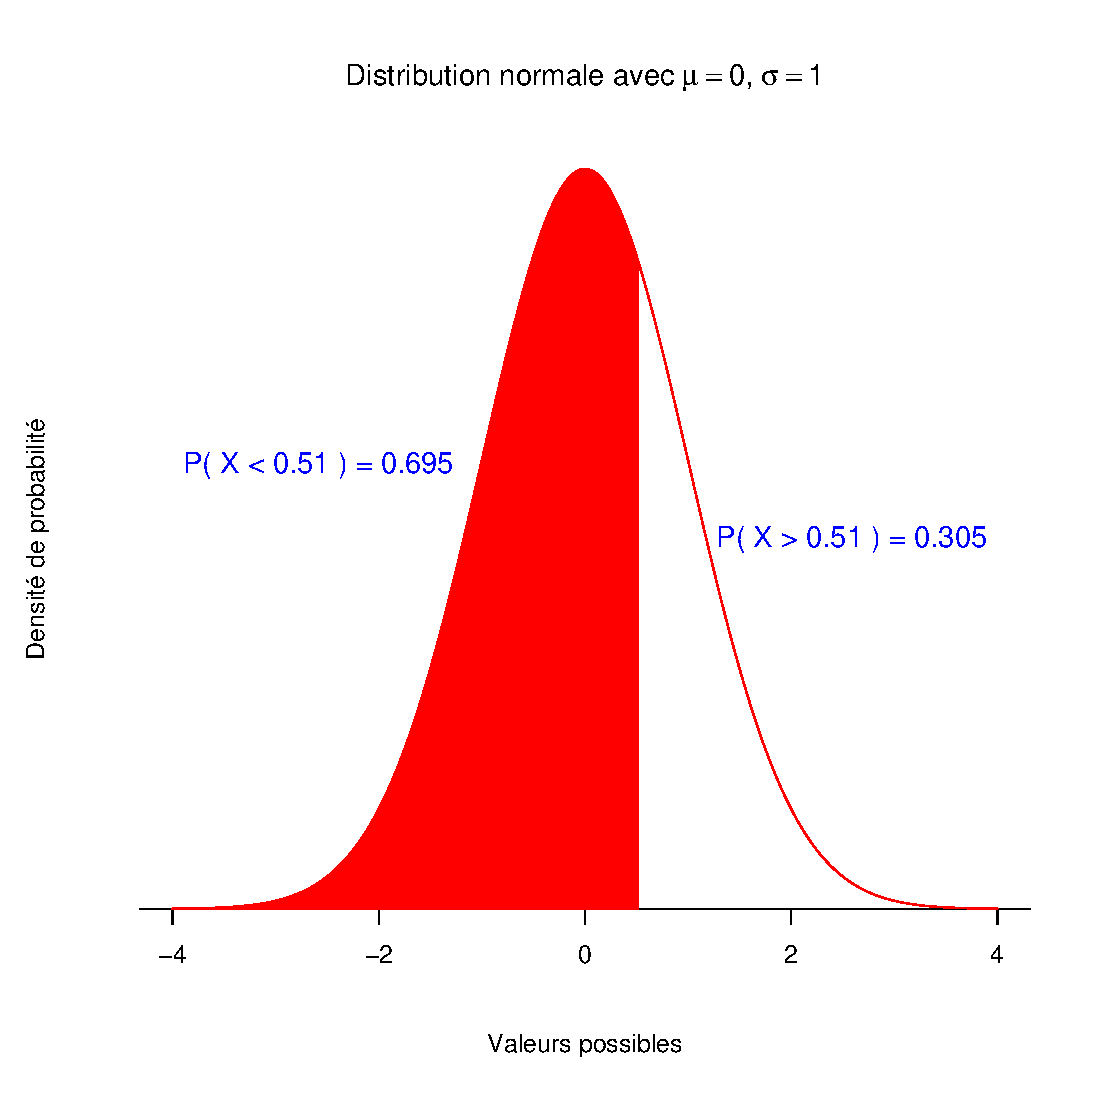
\includegraphics[scale=0.5]{norm_table}$$

En variant les param\`etres $\mu$ et $\sigma^2$ de la loi normale, nous obtenons diff\'erentes lois normales. Ainsi, il n'existe pas une seule loi normale, mais une multitudes de loi normales qui se diff\'erentient par leurs param\`etres.

$$
\includegraphics[scale=0.4]{normalesMu0}
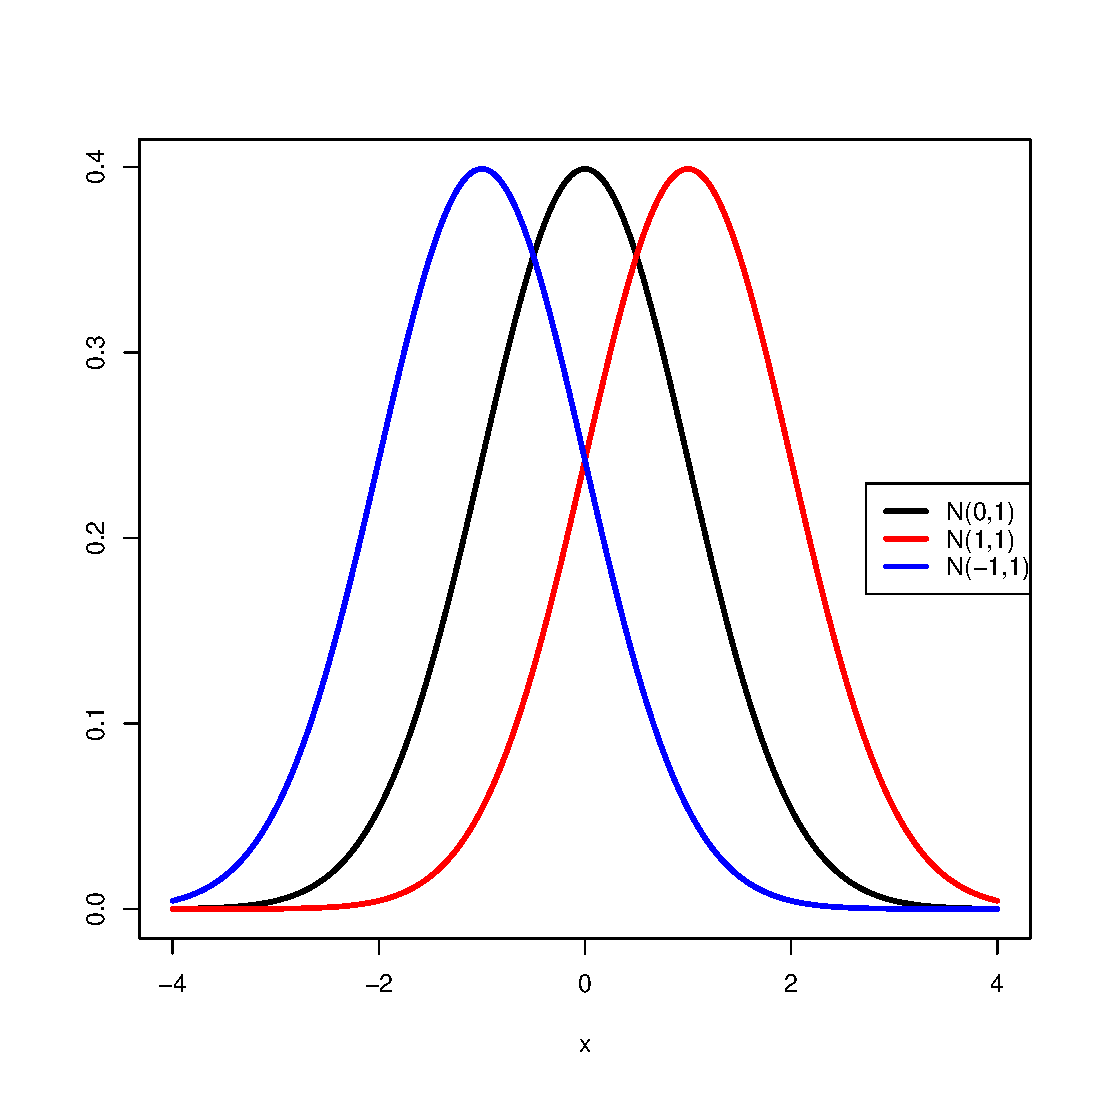
\includegraphics[scale=0.4]{normalesV1}$$

Il existe une distribution normale de r\'ef\'erence, de moyenne 0 et de variance 1, dite aussi distribution $Z$.

\begin{defi}
Une loi normale de moyenne nulle et d'\'ecart type 1 est dite \emph{loi normale centr\'ee r\'eduite}, aussi dite \emph{loi normale standard}. La fonction de densit\'e est alors
$$f(x)=\frac{1}{\sqrt{2\pi}}e^{-\frac{x^2}{2}}$$
\end{defi}

La lettre $Z$ est habituellement utilis\'ee pour d\'esigner la variable al\'eatoire continue dont la loi est normale centr\'ee r\'eduite. Il est toujours possible de transformer une variable al\'eatoire $X$ distribu\'ee selon une loi normale $\mathcal{N}(\mu,\sigma^2)$, en une variable $Z$ distribu\'ee selon une loi normale centr\'ee r\'eduite $\mathcal{N}(0,1)$. La transformation consiste \`a soustraire de $X$ la moyenne $\mu$, puis de diviser par l'\'ecart type $\sigma$
$$X\sim \mathcal{N}(\mu,\sigma^2)\quad\Rightarrow\quad Z=\frac{X-\mu}{\sigma}\sim\mathcal{N}(0,1)$$
Les probabilit\'es suivantes sont alors \'equivalentes, avec $X\sim\mathcal{N}(\mu,\sigma^2)$

$$X\leq x\quad\Rightarrow\quad Z\leq\frac{x-\mu}{\sigma}$$
$$P(X\leq x)=P(Z\leq\frac{x-\mu}{\sigma})$$

\begin{ex}
Si $X$ est une variable al\'eatoire suivant une loi normale de centre $\mu=100$ et d'\'ecart type $\sigma=50$, i.e. 
$$X\sim\norm (100,2500)$$ 
alors la $z$ valeur associ\'ee est 
$$Z=\frac{X-\mu}{\sigma}\sim\norm (0,1)$$
\vspace{5mm}

%$$
%	% \usepackage{pst-plot}
%\begin{pspicture}(-0.5,-1)(2.5,2.1)
%\psset{linewidth=0.5pt,xunit=3cm,yunit=3cm}
%\parametricplot[plotpoints=100]{-0.5}{2.5}{t 1 0.5 2 3.1416 mul sqrt mul div 2.71828 t 1 sub 2 exp 2 0.5 2 exp mul div neg exp mul}
%\psaxes[arrowscale=1.5,ticks=none,labels=none]{->}(-0.5,0)(2.5,1.0)
%\psline(1,-0.1)(1,0.1)
%\uput[90](1.0,-0.3){100}
%\uput[90](1.0,-0.45){\red 0}
%\psline(2.0,-0.1)(2.0,0.1)
%\uput[90](2.0,-0.3){200}
%\uput[90](2.5,-0.3){X}
%\uput[90](2.0,-0.45){\red 2}
%\uput[90](2.5,-0.45){\red Z}
%\uput[90](2,0.8){$X\sim\norm (100,2500)$}
%\uput[90](2,0.5){\red $Z\sim\norm (0,1)$}
%\end{pspicture}$$

%\newcommand{\sigma}{50}
%\newcommand{\moyenne}{100}
%% temporary off because of a bug of tikz
%\shorthandoff{:}
%$$
%\begin{tikzpicture}[scale=0.8, domain=0:4]
%\draw[->] (-0.2,0) -- (4.2,0);
%\draw[->] (0,-0.2) -- (0,4);
%%\draw plot (\x,{1/{\sigma*sqrt(2*pi)}*exp(-pow(\x-\moyenne,2)/{2*pow(\sigma,2)})}) ;
%\foreach \pos/\label in {1/100,2/200,3/300,4/X}
%        \draw (\pos,0) -- (\pos,-0.1) (\pos cm,-3ex) node
%            [anchor=base,fill=white,inner sep=1pt]  {\label};
%\foreach \pos/\label in {1/0,2/2,3/4,4/Z}
%        \draw [color=red] (\pos cm,-6ex) node
%            [anchor=base,fill=white,inner sep=1pt]  {\label};
%\node [right] at (2,3) {$X\sim\norm (100,2500)$};
%\node [right, color=red] at (2,2.3) {$Z\sim\norm (0,1)$};
%\end{tikzpicture}
%$$
%\shorthandon{:}

$$\includegraphics[scale=0.4]{Rnormal.pdf}$$

Ainsi, si $X=200$, alors $Z=\frac{200-100}{50}=2$. Cela signifie que $X=200$ est \'eloign\'e de 2 \'ecarts type au del\`a de la moyenne.\\
Nous avons alors $100+2*50 = 200 = X$
\end{ex}

\paragraph{Table de la loi normale}
La table de la loi normale donne les probabilit\'es d'occurrence jusqu'\`a la z-valeur consid\'er\'ee. La ligne donne la valeur de z jusqu'au dixi\`eme, et la colonne donne la valeur de z au centi\`eme.

\begin{ex}
\begin{itemize}
	\item La z-valeur associ\'ee \`a la ligne 0.5 et \`a la colonne 0.01 correspond \`a Z=0.51.\\
L'intersection de la ligne et de la colonne donne la probabilit\'e cherch\'ee:\\
$P(Z\leq 0.51)=0.6950$
  \item $P(Z\geq 0.51)=1-0.6950 = 0.305$ par compl\'ementarit\'e.
  \item $P(Z\leq -0.51) = P(Z\geq 0.51) = 0.305$ par sym\'etrie.
\end{itemize}
\end{ex}

\paragraph{R\`egle empirique}
En pratique, de nombreux ensembles de donn\'ees ont une distribution en forme de cloche. Dans ce cas, on peut utiliser une r\`egle empirique, fond\'ee sur une distribution de probabilit\'e normale:
\begin{itemize}
\item Environ 68\% des observations se situent dans l'intervalle $[\bar{x}-s;\bar{x}+s]$
\item Environ 95\% des observations se situent dans l'intervalle $[\bar{x}-2s;\bar{x}+2s]$
\item Environ 99.7\%  des observations (presque toutes) se situent dans l'intervalle\\ $[\bar{x}-3s;\bar{x}+3s]$
\end{itemize}

\vspace{5mm}
Les variables centr\'ees r\'eduites $Z$ permettent de d\'etecter des valeurs singuli\`eres de la mani\`ere suivante:
si les donn\'ees semblent \'etre le r\'esultat d'une variable al\'eatoire suivant une loi normale, presque toutes les observations devraient se trouver entre la moyenne et $\pm$ 3 \'ecarts type. Il est alors recommand\'e de consid\'erer toute observation dont la valeur de $Z$ se situe en dehors de cet intervalle comme \'etant singuli\`ere.
